\documentclass[12pt]{book}
 
\usepackage[margin=1in]{geometry}
\usepackage[utf8]{inputenc}
\usepackage{verbatim}
\usepackage{pgfplots}
    \pgfplotsset{compat=1.12,}
\usepackage{enumitem}
\usepackage{amsmath,amsfonts,amsthm,amssymb,graphicx,mathtools,hyperref}
\usepackage{wrapfig}
\usepackage[export]{adjustbox}
\usepackage{tikz}
\renewcommand\qedsymbol{$\blacksquare$}
\usetikzlibrary{positioning}
\rerenewcommand{\A}{\mathbb{A}}
\renewcommand{\B}{\mathbb{B}}
\renewcommand{\C}{\mathbb{C}}
\renewcommand{\D}{\mathbb{D}}
\renewcommand{\E}{\mathbb{E}}
\renewcommand{\F}{\mathbb{F}}
\renewcommand{\G}{\mathbb{G}}
\renewcommand{\Hb}{\mathbb{H}} %
\renewcommand{\I}{\mathbb{I}}
\renewcommand{\J}{\mathbb{J}}
\renewcommand{\K}{\mathbb{K}}
\renewcommand{\Lb}{\mathbb{L}} %
\renewcommand{\M}{\mathbb{M}}
\renewcommand{\N}{\mathbb{N}}
\renewcommand{\Ob}{\mathbb{O}} %
\renewcommand{\Pb}{\mathbb{P}} % 
\renewcommand{\Q}{\mathbb{Q}}
\renewcommand{\R}{\mathbb{R}}
\renewcommand{\Sb}{\mathbb{S}} % 
\renewcommand{\T}{\mathbb{T}}
\renewcommand{\U}{\mathbb{U}}
\renewcommand{\V}{\mathbb{V}}
\renewcommand{\W}{\mathbb{W}}
\renewcommand{\X}{\mathbb{X}}
\renewcommand{\Y}{\mathbb{Y}}
\renewcommand{\Z}{\mathbb{Z}}

\newcommand{\Ac}{\mathcal{A}}
\newcommand{\Bc}{\mathcal{B}}
\newcommand{\Cc}{\mathcal{C}}
\newcommand{\Dc}{\mathcal{D}}
\newcommand{\Ec}{\mathcal{E}}
\newcommand{\Fc}{\mathcal{F}}
\newcommand{\Gc}{\mathcal{G}}
\newcommand{\Hc}{\mathcal{H}} %
\newcommand{\Ic}{\mathcal{I}}
\newcommand{\Jc}{\mathcal{J}}
\newcommand{\Kc}{\mathcal{K}}
\newcommand{\Lc}{\mathcal{L}} %
\newcommand{\Mc}{\mathcal{M}}
\newcommand{\Nc}{\mathcal{N}}
\newcommand{\Oc}{\mathcal{O}} %
\newcommand{\Pc}{\mathcal{P}} % 
\newcommand{\Qc}{\mathcal{Q}}
\newcommand{\Rc}{\mathcal{R}}
\newcommand{\Sc}{\mathcal{S}} % 
\newcommand{\Tc}{\mathcal{T}}
\newcommand{\Uc}{\mathcal{U}}
\newcommand{\Vc}{\mathcal{V}}
\newcommand{\Wc}{\mathcal{W}}
\newcommand{\Xc}{\mathcal{X}}
\newcommand{\Yc}{\mathcal{Y}}
\newcommand{\Zc}{\mathcal{Z}}
\newcommand{\ita}[1]{\textit{#1}}
\newcommand{\com}[2]{#1\backslash#2}
\newcommand{\oneton}{\{1,2,3,...,n\}}
\newcommand\idea[1]{\begin{gather*}#1\end{gather*}}
\newcommand\ef{\ita{f} }
\newcommand\eff{\ita{f}}
\newcommand\proofs[1]{\begin{proof}#1\end{proof}}
\newcommand\inv[1]{#1^{-1}}
\newcommand\setb[1]{\{#1\}}
\newcommand\en{\ita{n }}
\newcommand{\vbrack}[1]{\langle #1\rangle}
\DeclareMathOperator{\ord}{ord}
\DeclareMathOperator{\Hom}{hom}
\DeclareMathOperator{\ker}{ker}
\DeclareMathOperator{\deg}{deg}

\theoremstyle{plain}
\newtheorem{theorem}{Theorem}[section]
\newtheorem{lemma}[theorem]{Lemma}
\newtheorem{proposition}[theorem]{Proposition}
\newtheorem*{corollary}{Corollary}

\theoremstyle{plain} % just in case the style had changed
\newcommand{\thistheoremname}{}
\newtheorem*{genericthm}{\thistheoremname}
\newenvironment{namedtheorem}[1]
  {\renewcommand{\thistheoremname}{#1}%
   \begin{genericthm}}
  {\end{genericthm}}

\theoremstyle{definition}
\newtheorem*{definition}{Definition}
\newtheorem{conjecture}{Conjecture}
\newtheorem{example}{Example}[chapter]
\newtheorem*{HW}{Homework}

\theoremstyle{remark}
\newtheorem*{remark}{Remark}
\newtheorem*{claim}{Claim}
\newtheorem*{note}{Note}

\renewcommand*{\proofname}{Proof}
 
\title{Ring Theory}
\author{Alec Zabel-Mena\\ \textbf{\underline{Text}} \\  
Herstein (1965). Topics in Algebra. Blaisdel Publishing Co.}
\date{\today}

\begin{document}

\maketitle

%----------------------------------------------------------------------------------------
%	CHAPTER X
%----------------------------------------------------------------------------------------

\chapter{Modules} % Main chapter title

\label{Chapter1} % Change X to a consecutive number; for referencing this chapter elsewhere, use \ref{ChapterX}

%% to include section files use the \input{} command.

%----------------------------------------------------------------------------------------
%	SECTION 1.1
%----------------------------------------------------------------------------------------

\section{Definitions and Examples}
\label{section1}

\begin{definition}
    We call a nonemty set $V$ a \textbf{vector space} over a field $F$, if given
    a binary operation  $+:V \times V \rightarrow V$ called \textbf{vector
    addition} and an operation $\cdot:F \times V \rightarrow V$ called
    \textbf{scalar multiplication}, we have that $(V,+)$ forms an abelian group,
    and for all $v,w \in V$ and  $\alpha,\beta \in F$:
     \begin{enumerate}[label=(\arabic*)]
         \item $\alpha(v+w)=\alpha v+\alpha w$.

         \item $ (\alpha+\beta)v=\alpha v+\beta v$.

         \item $\alpha(\beta v)=(\alpha\beta)v$.

         \item $1v=v$, where  $1$ as the identity element of  $F$ under its
             multiplication.
    \end{enumerate}
\end{definition}

\begin{lemma}\label{1.1.1}
    Let $V$ be a vector space over a field  $F$. Then the operation  $\cdot:F
    \times V \rightarrow V$ of scalar mutliplication as a group homomorphism of
    $V$ into  $V$.
\end{lemma}
\begin{proof}
    Taking $\cdot:F \times V \rightarrow V$ by $(\alpha,v) \rightarrow \alpha
    v$, restrict $\cdot$ to  $V$, i.e. consider $\cdot|_{V}:V \rightarrow V$ by
    $v \rightarrow \alpha v$ for $\alpha \in F$. By $(1)$ of the scalar
    multiplication rules, we get that $\cdot|_{V}$ as a homomorphism; which
    makes $\cdot$ a homomorphism.
\end{proof}

\begin{example}
    \begin{enumerate}[label=(\arabic*)]
        \item Let $F$ be a field and  $F \subseteq K$ a field extension of  $F$.
            Then  $K$ as a vector space over  $F$ with  $+$ the usual addition
            of  $K$ and  $\cdot$ the multiplication of  $K$ restricted to  $F$
            by the first part, i.e. the product  $\cdot:v \rightarrow \alpha v$
            with $\alpha \in F$.

        \item Let  $F$ be a field and consider  $F^n$ the set of ordered
            $n$-tuples of elements of $F$, for some  $n \in \Z^+$. Take $+:(v,w)
            \rightarrow v+w$ by $(v_1, \dots, v_n)+(w_1, \dots, w_n)=(v_1+w_1,
            \dots, v_n+w_n)$, where $v=(v_1, \dots, v_n), w=(w_1, \dots, w_n)
            \in F^n$, and $\cdot:(\alpha,v) \rightarrow \alpha v$ by
            $\alpha(v_1, \dots, n_n)=(\alpha v_1, \dots, \alpha v_n)$. Then
            $F^n$ as a vector space over  $F$.

        \item Let  $F$ be any field and let  $F[x]$ be the polynomial field over
            $F$. Take  $+$ to be polynomial addition, and  $\cdot$ the
            multiplication of a constant in $F$ by a polynomial in $F[x]$. Then
            $F[x]$ as a vector space over $F$.

        \item LEt  $F[x]$ be the polynomial field over a field $F$ and consider
            the set  $P_n=\{f \in F{x}: \deg{f}<n\}$. Then $P_n$ as a subset of
             $F[x]$ forms a vector space over $F$ under the same operations  $+$
             and  $\cdot$ (thas last example motivates the following
             definition).
    \end{enumerate}
\end{example}

\begin{definition}
    LEt $V$ be a vector space over a field  $F$. We say a subset  $W \subseteq
    V$ as a \textbf{subspace} of $V$ if  $W$ as also a vector space over $F$.
\end{definition}

\begin{lemma}\label{1.1.2}
    Let $V$ be a vector space over a field  $F$, and let  $W \subseteq V$ be a
    subspace of  $V$. Then for all  $ w_1,w_2 \in W$ and $\alpha,\beta \in F$,
    $\alpha w_1+\beta w_2 \in W$.
\end{lemma}
\begin{proof}
    Since $W$ as a vector space  we have that $ \alpha w_1,\beta w_2 \in W$;
    then by closure of vector addition, $\alpha w_1+\beta w_2 \in W$.
\end{proof}

\begin{definition}
    Let $U$ and  $V$ be vector spaces over a filed  $F$. We call a mapping  $T:U
    \rightarrow V$ a \textbf{homomorphism} of $U$ into  $V$ if: 
        \begin{enumerate}[label=(\arabic*)]
            \item $T(u_1+u_2)=T(u_1)+T(u_2)$.

            \item $T(\alpha u_1)=\alpha T(u_1)$.
        \end{enumerate}
    for all $ u_1,u_2 \in U$ and $\alpha \in F$. If  $T$ as  $1-1$ from  $U$
    onto  $V$, then we call  $T$ an \textbf{isomorphism} and we say $U$ as
    \textbf{ismorphic} to $V$ and write  $U \simeq V$. We define the
    \textbf{kernal} of $T$ to be  $\ker{T}=\{u \in U: T(u)=0\}$. We call the set
    of all homomorphism of $U$ into  $V$  $\hom(U,V)$.
\end{definition}

\begin{example}
    Let $F$ be a field and consider the vector spaces  $F^n$ and  $P_n$ defined
    in examples $(2)$ and $(4)$. Then $P_n \simeq F^n$. Take the map  $
    a_0+a_1x+\dots+a_nx^{n-1} \rightarrow (a_0, \dots, a_{n-1})$, which defines
    an isomorphism.
\end{example}

\begin{lemma}\label{1.1.3}
    If $V$ as a vector space over a field  $F$, then for all  $\alpha \in F$ and
     $v \in V$:
        \begin{enumerate}[label=(\arabic*)]
            \item \alpha0=0.

            \item $0v=0$.

            \item $(-\alpha)v=-(\alpha v)$.

            \item $\alpha v=0$ and $v \neq 0$ implies $\alpha=0$.
        \end{enumerate}
\end{lemma}
\begin{proof}
    \begin{enumerate}[label=(\arabic*)]
        \item $\alpha0=\alpha(0+0)=\alpha0+\alpha0$, hence $\alpha0=0$.

        \item $0v=(0+0)v=0v+0v$, hence $0v=0$.

        \item He have $0=0v$, that as $0=(\alpha+(-\alpha))v=\alpha
            v+(-\alpha)v$. Adding both sided by $-(\alpha v)$ we get the desired
            result.

        \item If  $\alpha \neq 0$ and $v \neq 0$, then $0=\alpha^{-1}0=\alpha^{-1}(\alpha v)=1v=v$
            which makes $v=0$, which cannot happen. So $\alpha=0$.
    \end{enumerate}
\end{proof}

\begin{lemma}\label{1.1.4}
    Let $V$ be a vector space over a field  $F$ and let  $W \subseteq V$ be a
    subspace of  $V$. Then  $V/W$ as a vector space over  $F$ where for $
    v_1+W,v_2+W \in V/W$ and $\alpha \in F$ we have:
        \begin{enumerate}[label=(\arabic*)]
            \item $(v_1+W)+(v_2+W)=(v_1+v_2+W)$.

            \item $\apha(v_1+W)=\alpha v_1+W$.
        \end{enumerate}
\end{lemma}
\begin{proof}
    Since $V$ as an abelian group, and  $W$ a subgroup of  $V$ under  $+$, we
    get that  $V/W$ as the quotient group of  $V$ over  $W$; which as abelian
    since  $W$ as abelian.

    Suppose now that for $v,v' \in V$ that  $v+W=v'+W$, then for  $\alpha \in F$
    we have  $\alpha(v+W)=\alpha(v'+W)$, and by hypotheses, we have $v-v' \in
    W$. Now since  $W$ as a subspace,  $\alpha(v-v') \in W$ as well, so $\alpha
    v+W=\alpha v'+W$, so the product as well defined.

    Now consider  $v,v' \in W$ and  $\alpha, \beta \in F$. By our product we
    have that  $\alpha(v+w+W)=\alpha(v+w)+W=(\alpha v+ \alpha w)+W=(\alpha
    v+W)+(\alpha v'+W)$, $(\alpha+\beta)(v+W)=(\alpha+\beta)v+W=(\alpha v+\beta
    v)+W=\alpha(v+W)+\beta(v+W)$, $\alpha(\beta v+W)=\alpha\beta v+W=(\alpha\beta)
    v+W$, and finally, $1(v+w)=1v+W=v+W$. Therefore $V/W$ as a vector space over
     $F$.
\end{proof}

\begin{definition}
    Let $V$ be a vector space over  $F$ and let  $W \subseteq V$ be a subspace
    of  $V$. We call the vector space formed by taking the quotient group of
    $V$ over  $W$,  $V/W$ the  \textbf{quotient space} of $V$ over  $W$.
\end{definition}

\begin{theorem}[The First Homomorphism Theorem for Vector Spaces]\label{1.1.5}
    If $T:U \rightarrow V$ as a homomorphism of $U$ onto  $V$, and  $W=\ker{T}$,
    then $V \simeq U/W$. If  $U$ as a vector space and  $W \subseteq U$ as a
    subspace of  $U$, then  there as a homomorphism of  $U$ onto  $U/W$.
\end{theorem}
\begin{proof}
    By the fundamental theorem of homomorphisms, we have that, as groups, $V
    \simeq U/W$. That there as a homomorphism from  $U$ onto  $U/W$ follows
    immediately.
\end{proof}

\begin{definition}
    Let $V$ bhe a vector space over a field  $F$ and let  $\{U_i\}_{i=1}^n$ be a
    collection of subspaces of $V$. We call $V$ the \textbf{internal direct
    sum} of $\{U_i\}$ if every element of $V$ can be written uniquely as a 
    vector sum of elements of each $U_i$ for $1 \leq i \leq n$; That as  for 
    $v \in V$, $v=u_1+\dots+u_n$ as unique where $u_i \in U_i$.
\end{definition}

\begin{lemma}\label{1.1.6}
    Let $\{V_i\}_{i=1}^n$ be a collection of vector spaces over a field $F$ and
    let  $V=\prod_{i=1}^n{V_i}$ and define $+:V \times V \rightarrow V$ by
    $(v_1, \dots, v_n)+(v_1', \dots, v_n')=(v_1+v_1', \dots, v_n+v_n')$ and
    define $\cdot:F \times V \rightarrow V$ by $\alpha(v_1, \dots, v_n)=(\alpha
    v_1, \dots, \alpha v_n)$. Then $V$ as a vector space over  $F$.
\end{lemma}
\begin{proof}
    Since $V_i$ as a vector space for all  $1 \leq i \leq n$, they are all
    abelian groups, hence  $V$ as closed under  $+$, and inherits associativity,
    as well a s commutativity. Now letting  $0=(0_1, \dots, 0_n)$, where $0_i$ 
    as the identity of  $V_i$, we get for any  $v \in V$ that  $v+0=o+v=v$, so  
    $0$ as the identity. Likewise for any  $v \in V$,  $-v=(-v_1, \dots, -v_n)$
    serves as the inverse for $v$. So  $(V,+)$ forms an abelian group.

    Now by the axioms of scalar multiplication on each of the $V_i$, let
    $v=(v_1, \dots, v_n),w=(w_1, \dots, w_n) \in V$ and $\alpha,\beta \in F$. We
    get  $\alpha(v+w)=\alpha(v_1+w_1, \dots v_n+w_n)=(\alpha(v_1+w_1), \dots,
    \alpha(v_n+w_n))=(\alpha v_1+\alpha w_1, \dots, \alpha v_n+\alpha
    w_n)=(\alpha v_1, \dots, \alpha v_n)+(\alpha w_1, \dots, \alpha w_n)=\alpha
    v+\alpha w$. We also get $(\alpha+\beta)v=((\alpha+\beta)v_1, \dots,
    (\alpha+\beta)v_n)=(\alpha v_1+\beta v_1, \dots, \alpha v_n+\beta
    v_n)=(\alpha v_1, \dots, \alpha v_n)+(\beta v_1, \dots, \beta v_n)=\alpha
    v+\beta v$. Through similar calculation, we get that $\alpha(\beta
    v)=(\alpha\beta)v$ and $1v=v$; which makes  $V$ into a vector space.
\end{proof}

\begin{definition}
    Let $\{V_i\}_{i=1}^n$ be a collection of vector spaces over a field $F$ and
    let  $V=\prod_{i=1}^n{V_i}$ and define $+:V \times V \rightarrow V$ by
    $(v_1, \dots, v_n)+(v_1', \dots, v_n')=(v_1+v_1', \dots, v_n+v_n')$ and
    define $\cdot:F \times V \rightarrow V$ by $\alpha(v_1, \dots, v_n)=(\alpha
    v_1, \dots, \alpha v_n)$. We call $V$, as a vector space over  $F$ the
    \textbf{external direct sum} of $\{V_i\}$ and write $V=V_1 \oplus \dots
    \oplus V_n$, or $V=\bigoplus_{i=1}^n{V_i}$.
\end{definition}

\begin{theorem}\label{1.1.7}
    Let $V$ be a vector space and let  $\{U_i\}_{i=1}^n$ be a collection of
    subspaces of $V$. If $V$ is the internal direct sum of  $\{U_i\}$ then $V$
    is isomorphic to the external direct sum of  $\{U_i\}$; that is: $V
    \simeq \bigoplus_{i=1}^n{U_i}$.
\end{theorem}
\begin{proof}
    Let $v \in V$. By hypothesis $v=u_1+\dots+u_n$ with $u_i \in U_i$ for  $1
    \leq i \leq n$, and it is a unique representation of  $v$. Define then, the
    map  $T:V \rightarrow \bigoplus_{i=1}^n{U_i}$ by the map $v=v=u_1+\dots+u_n
    \rightarrow (u_1, \dots, u_n)$. Since $v$ has a unique representation by
    definition,  $T$ is well defined; moreover it is $1-1$, as $(u_1, \dots,
    u_n)=(w_1, \dots w_n)$ implies $u_i=w_i$ for all  $1 \leq i \leq n$, hence
    $ u_1+\dots+u_u=w_1+\dots+w_n$, and since this sum is unique, they both
    represent a vector $v \in V$. That  $T$ is onto follows directly from
    definition.

    Finally, let  $v,w \in V$, then  $v=u_1+\dots+u_n$ and $w=w_1+\dots+w_n$.
    Hence $T(v+w)=T(u_1+w_1+\dots+u_n+w_n)=(u_1+w_1, \dots, u_n+w_n)=(u_1,
    \dots, u_n)+(w_1, \dots, w_n)=T(v)+T(w)$. Similarly, $T(\alpha
    v)=\alphaT(v)$.
\end{proof}
\begin{remark} 
    That $V$ is the internal direct sum of  $\{U_i\}$ and that $V \simeq U_1 \oplus
    \dots \oplus U_n$ by the above theorem permits us to write $V=U_1 \oplus
    \dots \oplus U_n$, or $V=\bigoplus_{i=1}^n{U_i}$.
\end{remark}

%----------------------------------------------------------------------------------------
%	SECTION 1.1
%----------------------------------------------------------------------------------------

\section{Connected Spaces of The Real Line.}

\begin{definition}
    We call a simply ordered set $L$ with  $|L|>1$ a  \textbf{ordered contunuum} if:
        \begin{enumerate}[label=(\arabic*)]
            \item $L$ has the least upperbound property.

            \item If $x<y$, then there exists a  $z$ such that  $x<z<y$.
        \end{enumerate}
\end{definition}

\begin{theorem}\label{3.2.1}
    If $L$ is a linear continuum in the order topology, then  $L$ is connected, and so are the open
    sets of  $L$  (the intervals and rays in $L$).
\end{theorem}
\begin{proof}
    We show that convex sets are connected. Let $Y=A \cup B$ be a seperation, and choose  $a \in A$,
     $b \in B$ with  $a<b$. We have that the interval of points in  $L$,  $[a,b] \subseteq Y$; and
     we also have that $[a,b] \subseteq A_0 \cup B_0$ with $ A_0=A \cap [a,b]$ and $ B_0=B \cap
     [a,b]$. Now $ A_0,B_0 \neq \emptyset$, so $[a,b]=A_0 \cup B_0$ is a seperation of $[a,b]$. Now
     let $c=\sup{A_0}$. Suppose first that $c \in B_0$, then $c \neq a$, so either $c=b$ or  $a<c<b$.
     Since  $ B_0$ is open in $[a,b]$ as a subspace of $Y$, there is some interval  $(d,c] \subseteq
     B_0$.

     If $c=b$, then  $d<c$ is an upperbound of  $ A_0$, which contradicts that $c$ is the least
     upperbound. Now suppose that $c<b$. We have that since  $c,b \in B_0$, $(c,b] \cap A_0=
     \emptyset$, then $(b,d] \cap A_0=(d,c] \cap (c,b] \cap A_0 = \emptyset$, and again we have
     $d<c$ which gives us the contradiction. So  $c \notin B$. By similar reasoning  $c \notin A_0$.
\end{proof}
\begin{corollary}
    $\R$ is connected and so are the intervals and rays of  $\R$.
\end{corollary}
\begin{proof}
    $\R$ is a linear continuum.
\end{proof}

\begin{theorem}[The Intermediate Value Theorem]\label{3.2.2}
    Let $f:X \rightarrow Y$ be continuous with  $X$ connected, and  $Y$ an ordered set under the
    order topology. If  $a,b \in X$, and if  $r \in Y$ such that  $f(a)<r<f(b)$ or $f(b)<r<f(a)$,
    then there exists a $c \in X$ for which  $f(c)=r$.
\end{theorem}
\begin{proof}
    Let $r \in Y$ such that  $f(a)<r<f(b)$, without loss of generality. We have that $A=f(X) \cap
    (-\infty, r)$ and $B=f(X) \cap (r ,\infty)$ are disjoint, nonempty sets open if $f(X)$ as a
    subspace of $Y$. Now suppose there is no  $c \in X$ for which  $f(c)=r$, then $f(X)=A \cup B$ is
    a seperation of $f(X)$, which contradicts theorem \ref{3.1.6}.
\end{proof}

\begin{example}
    \begin{enumerate}[label=(\arabic*)]
        \item The ordered square $I_0^2$ is a linera continuum. Let $A \subseteq I_0^2$ and consider
            the projection $\pi_1:I_0^2 \rightarrow I_0^2$. Let $b=\sup{\pi_1(A)}$, now if $b \in
            \pi_1(A)$ then $A \cap (b \times I_0) \neq \emptyset$, and since $I_0 \subseteq \R$, $A
            \cap (b \times I_0)$ has a least upperbound, $b \times c$, where  $c=\sup{I_0}$, which
            is also the least upperbound of $A$. Now if we have $a \times c < b \times d$, then
            $a<b$ and  $c<d$; and since  $\R$ is a linear continuum, there are $y,z \in \R$ for
            which  $a<y<b$ and  $c<z<d$. Hence  $a \times c < y \times z < b \times d$; which makes
            $ I_0^2$ into a liear continuum.

        \item If $X$ is a well ordered set, then  $X \times [0,1)$ is a linear contiuum in the
            dictionary order. Let $A \subseteq X \times [0,1)$ and consider the projection $\pi_2:X
            \times [0,1) \rightarrow [0,1)$. If $b=\sup{\pi_2(A)}$, then $A \cap (b \times [0,1)) \neq
            0$, and so $A \cap (b \times [0,1)$ has a least upperbound $b \times c$ with
            $c=\sup{[0,1)}$, which is also a least upperbound of $A$.

            Now since $\R$ is a linear continuum, if $x \times a < y \times b$, under the dictionary
            order, then  $x \leq y$ and  $a<b$. Then there are  $c,z \in \R$ such that  $x \leq z
            \leq y$ and  $a<c<b$, so that $x \times a < z \times c < y \times b$.
    \end{enumerate}
\end{example} 

\begin{definition}
    Let $X$ be a topological space with  $x, y \in X$. A \textbf{$xy$-path} in $X$ from  $x$ to  $y$ is a
    continuous map  $f:[a,b] \rightarrow X$, with $[a,b] \subseteq \R$ such that $f(a)=x$, and
    $f(b)=y$. We call $X$ \textbf {path connected} if there exists an $xy$-path in $X$ for every
    $x,y \in X$.
\end{definition}

\begin{theorem}\label{3.2.3}
    Path connected spaces are connected
\end{theorem}
\begin{proof}
    Let $X$ be path connected, and suppose that  $X=A \cup B$ is a seperation of  $X$. Let  $f:[a,b]
    \rightarrow X$ be some path in $X$. Since  $f$ is continuous, and  $[a,b] \subseteq \R$, by
    theorem \ref{3.1.6}, $f([a,b]) \subseteq X$ is a connected subspace, so either $f([a,b])
    \subseteq A$ or $f([a,b]) \subseteq B$, so there is no path from a point in $A$ to a point in
    $B$. But  $X$ is path connected; a contradiction. Therefore  $X$ must be connected.
\end{proof}

\begin{example}
    \begin{enumerate}[label=(\arabic*)]
        \item Define the \textbf{unit ball} in $\R^n$ under  $||\cdot||$ to be  $B^n=\{x \in
            \R^n:||x|| \leq 1\}$. $B^n$ is path connected. Consider  $f[0,1] \rightarrow B^n$ by
            $f(t)=(1-t)x+ty$, then $||f(t)||=(1-t)||x||+t||y|| \leq 1$, hence $f(t) \in  B^n$.
            Extending this to arbitrariy balls, for $\epsilon>0$, $B(x,\epsilon)$ and
            $cl{B(x,\epsilon)}$ are also path connected. The function $f$ also shows that the unit
            ball, and open balls  (as well as their closure) are convex.

        \item Define \textbf{punctured Euclidean space} to be $\com{\R^n}{\{0\}}$. If $n>1$,
        $\com{\R}{\{0\}}$ is path connected. Connect the points $x,y \in \com{\R^n}{\{0\}}$ by a
        straight line not passing through $0$, or choose a point $z \in \com{\R^n}{\{0\}}$ on that
        line and form a path by adjoining the lines from $x$ to  $z$ and from  $z$ to  $y$

        \begin{figure}[h] 
            \centering
            
\includegraphics[scale=0.2]{Figures/Chapter3/puncturedSpace.eps}
            \caption{Punctures $2$-space $\com{\R^2}{\{0\}}$.}
            \label{fig_3.1}
        \end{figure}

    \item Consider the unit sphere $S^{n-1}=\{x \in \R^n:||x||=1\}$ in $\R^n$.  $S^{n_-1}$ is path
        connected for $n>1$. Take the map  $g:\com{\R^n}\{0\} \rightarrow S^{n-1}$ by $g:x
        \rightarrow \frac{x}{||x||}$.

    \item The ordered square $ I_0^2$ is connected, but it is not path connected/ Let $p=0 \times
        0$,  $1=1 \times 1$ and let  $f:[a,b] \rightarrow I_0^2$ be a path joining $p$ and  $q$. We
        have that  $f([a,b])$ must contain all $x \times y \in I_0^2$ by the intermediate value
        theorem. Hence for each  $x \in I_0$, $U_x=f^{-1}(x \times I_0) \neq \emptyset$ and it is
        also open in $[a,b]$. Now choose for each $x \in I_0$, $q_x \in \Q$ such that  $q_x \in
        U_x$. Since  $\bigcap_{x \in I_0}{U_x} = \emptyset$, the map $x \rightarrow q_x$ is  $1-1$
        of  $I_0$ onto $\Q$. which makes $I_0$ countable; a contradiction.

    \item 
        \begin{figure}[h]
            \centering
            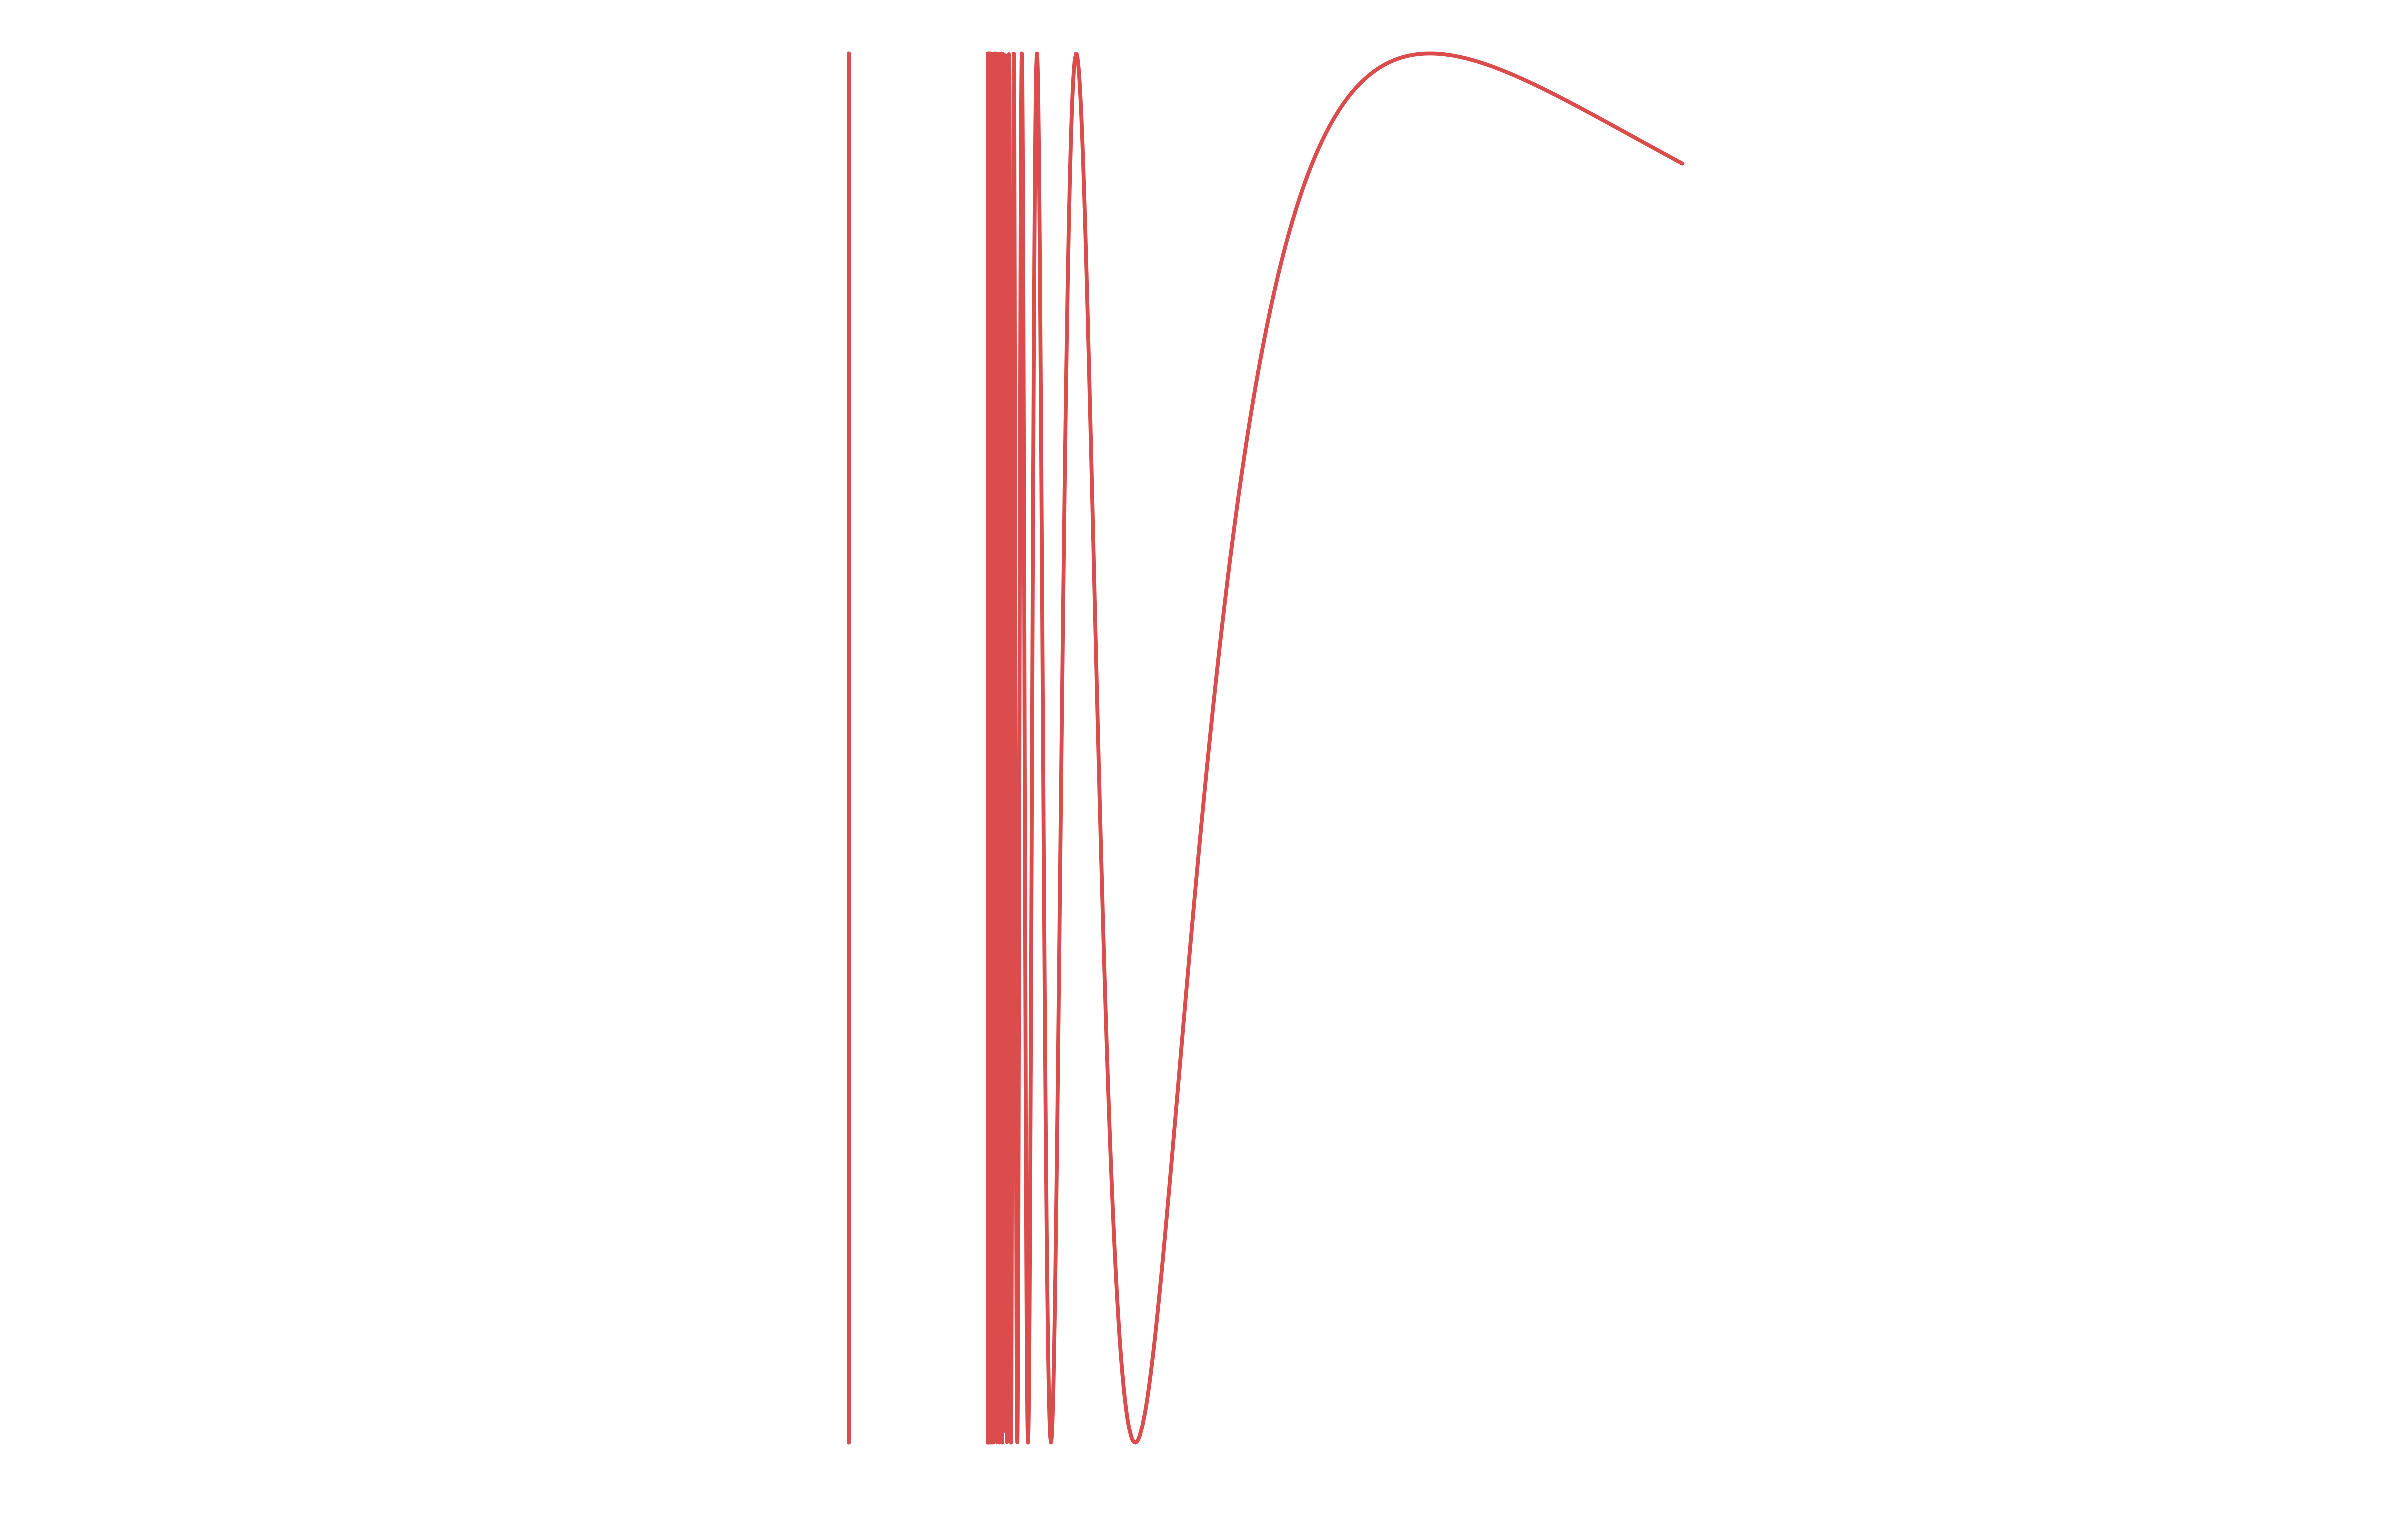
\includegraphics[scale = 0.2]{Figures/Chapter3/topologistsSineCurve.eps}
            \caption{The topologists Sine Curve, defined by $x \times \sin{\frac{1}{x}}$.}
            \label{fig_3.2}
        \end{figure}

        Let $S=\{x \times \sin{\frac{1}{x}}:0 < x \leq 1\}$. This is the image of the continuous map
        $x \rightarrow x \times \sin{\frac{1}{x}$ from $(0,1] \rightarrow \R^2$, Since $(0,1]$ is
            connected, then so is $S$. by theorem \ref{3.1.6}. We call $\cl{S}=S \cup (0 \times
            [-1,1])$ the \textbf{topologist's sine curve} (see figure \ref{fig_3.2}).

            Suppose that $f:[a,c] \rightarrow \cl{S}$ is a path begining at $0$ and ending at a
            point in  $S$. The set  $T=\{t \in \R:f(t) \in 0 \times [-1,1]\}$ is closed, so it has a
            largest element $b$. Then  $f$ is a path mapping  $b \rightarrow 0 \times [-1,1]$ and
            taking all other points to $S$. Suppose that  $[b,c]=[0,1]$ and let $f(t)=(x(t),y(t))$
            where $x(0)=0$, $x(t)>0$ and $y(t)=\sin{\frac{1}{x(t)}}$ for all $t>0$. For  $n \in
            \Z^+$, choose  $0<u<x(\frac{1}{n})$ such that $\sin{\frac{1}{u}}=(-1)^n$. By the
            intermediate value theorem, there are $0<t_n<\frac{1}{n}$ with $x(t_n)=u$. Then the
            sequence $\{t_n\} \rightarrow 0$, and $x(t_n)=(-1)^n$, which diverges; a contradiciton
            since $x(0)=0$ and $\{t_n\} \rightarrow 0$. Hence $\cl{S}$ is not path connected.

    \end{enumerate}
\end{example} 

%----------------------------------------------------------------------------------------
%	SECTION 1.1
%----------------------------------------------------------------------------------------

\section{Components and Local Connectedness.}

\begin{proposition}\label{3.3.1}
    Let $\sim$ be a relation defined on the topological space  $X$ by:  $x \sim y$ if there exists a
    connected subspace containing both  $x$ and  $y$. Then $\sim$ is an equivalence relation on
    $X$.
\end{proposition}
\begin{proof}
    Clearly, $x \sim x$. Now suppose that  $x \sim y$, then there is a connected subspace containing
    both  $x$ and  $y$, by definition,  $y \sim x$. Now suppose that  $x \sim y$ and  $y \sim z$.
    Then there are connected subspaces  $U$ and  $V$ with  $x,y \in U$,  $y,z \in V$. Since $y \in U
    \cap V$, by theorem \ref{3.1.4}, $U \cup V$ is a connected subspace with  $x,z \in U \cup V$.
    That is  $x \sim z$. 
\end{proof}

\begin{definition}
    Let $X$ be a topological space. Define an equivalence relation  $\sim$ on  $X$ by taking  $x
    \sim y$ if there is a onnected subspace of  $X$ containing  $x$ and  $y$. We call the
    equivalence classes of  $X/\sim$  \textbf{connected components} (or \textbf{components}) of
    $X$.
\end{definition}

%----------------------------------------------------------------------------------------
%	SECTION 1.1
%----------------------------------------------------------------------------------------

\section{Compact Spaces.}

\begin{definition}
    A collection $\Ac=\{A_{\alpha}\}$ of subsets of a topological space $X$ is said to be a  \textbf{cover}, or a
    \textbf{covering} of $X$ if  $\bigcup{A}=X$. We call $\{A\}$ an \textbf{open cover} if each $A$
    is open in  $X$. If  $\{A'\}$ is a subcollection of $\Ac$ that also covers $X$, we call
    $\{A'\}$ a \textbf{subcover} of $X$.
\end{definition}

\begin{definition}
    We call a topological space $X$ \textbf{compact} if for every open cover of $X$, there is a
    finite subcover of $X$.
\end{definition}

\begin{example}
    \begin{enumerate}[label=(\arabic*)]
        \item     $\R$ is not compact. Consider the following cover of  $\R$:
            \begin{equation*}
                \Ac=\{(n,n+2):n \in \Z\}
            \end{equation*}
            however, there is no finite subcollection of $\Ac$ that is a subcover of  $\R$.

        \item The subspace $X=\{0\} \cup \{\frac{1}{n}: n \in \Z\}$ of $\R$ is compact. Let  $\Ac$
            be a cover of  $X$. There is a  $U \in \Ac$ with  $0 \in U$ and $U$ contains all but
            finitely many of the points  $ \frac{1}{n}$. Now choose for each $\frac{1}{n} \in
            \com{X}{U}$ an element of $\Ac$ $A_{n}$ containing it. Then for all $n$,  $\{A_n\}$ is
            finite and covers $X$.

        \item If  $X$ is a finite topological space, then it is compact, since every open cover of
            $X$ is finite.

        \item The interval  $(0,1]$ is not compact. The open cover $\Ac=\{(\frac{1}{n}, 1]: n \in
            \Z^+\}$ contains no finite subcollection of $\Ac$ that covers  $(0,1]$. Likewise,
            $(0,1)$ is not compact by the same argument. However, $[0,1]$ is compact.
    \end{enumerate}
\end{example} 

\begin{lemma}\label{3.4.1}
    Let $Y$ be a subspace of a topological space  $X$.  $Y$ is compact if and only if every open
    cover of  $Y$, by open sets of  $X$ has a finite subcover of $Y$.
\end{lemma}
\begin{proof}
    Suppose $Y$ is compact and let  $\{A_\alpha\}$ be a cover of $Y$ with  $A_\alpha$ open in  $X$
    for all  $\alpha$. Since  $\{A_\alpha\}$ covers $Y$, so does the collection  $\{A_\alpha \cap
    Y\}$, where $A_\alpha \cap Y$ is open in  $Y$ for all  $\alpha$. Since  $Y$ is compact, choose
    the finite subcollection  $\{A_i \cap Y\}_{i=1}^{n}$ to be a finite subcover of $Y$; i.e.
    $\{A_i \cap Y\}_{i=1}^{n} \subseteq \{A_\alpha\}$.

    Conversely, suppose that for every cover $\{A_\alpha\}$, open in  $X$, of  $Y$ that
    $\{A_\alpha\}$ contains a finite subcover of $Y$. Choose  $A_\alpha'=A_\alpha \cap Y$ for all
    $\alpha$; then $\{A_\alpha'\}$ is an open cover of $Y$. 
    By hypthesis, there is a finite subcover $\{A_i\}_{i=1}^n$, and by our assignment, we
    get that $\{A_i'\}_{i=1}^n \subseteq \{A_\alpha'\}$ is also a finite subcover of $Y$. Therefore
     $Y$ is compact as a subspace of  $X$.
\end{proof}

\begin{theorem}\label{3.4.2}
    Every closed subspace of a compact space is compact.
\end{theorem}
\begin{proof}
    Let $Y$ be a closed subspace of a compact space $X$. Let $\{A_\alpha\}$ be an open cover of $Y$
    with  $A_\alpha$ open in  $X$ for all  $\alpha$. Consider  $\{B_\alpha\}=\{A_\alpha\} \cup
    \com{X}{Y}$. Since $\{A_\alpha\}$ covers $Y$,  $\{B_\alpha\}$ covers $X$. Now take some finite
    subcollection  $\{B_i\}_{i=1}^n$. If it contains $\com{X}{Y}$, then just consider
    $\com{\{B_i\}}{(\com{X}{Y})}$. Then this collection is a finite subcover of $Y$.
\end{proof}

\begin{theorem}\label{3.4.3}
    Every compact subspace of a Hausdorff space is closed.
\end{theorem}
\begin{proof}
    Let $Y$ be a compact subsapce of a Hausdorff space  $X$. Choose  $x_0 \in \com{X}{Y}$ and for
    each $y \in Y$ choose disjoint neighborhoods  $U_y$ and  $V_y$ of  $ x_0$ and $y$ respectively.
    The collection  $\{V_y\}$ covers $Y$ by open sets in  $X$, hence there is a finite subcover, by
    theorem \ref {3.4.2}, $\{V_{y_n}\}$ of $Y$. Take  $V=\bigcup_{i=1}^n{V_{y_i}}$ to be open in
$X$, and take  $U=\bigcap_{i=1}^n{U_{y_i}}$ also open in $X$. Then  $Y \subseteq V$ and  $V \cap
U=\emptyset$; for take $z \in V$,  $z \in V_{y_i}$ for some $1 \leq i \leq n$. Hence  $z \notin
U_{y_i}$, so $z \notin U$. Then  $U$ is a neighborhood of  $X$, disjoint from  $Y$, making
$\com{X}{Y}$ open in $X$. Therefore  $Y$ is closed in  $X$.
\end{proof}

\begin{figure}[h] 
    \centering
    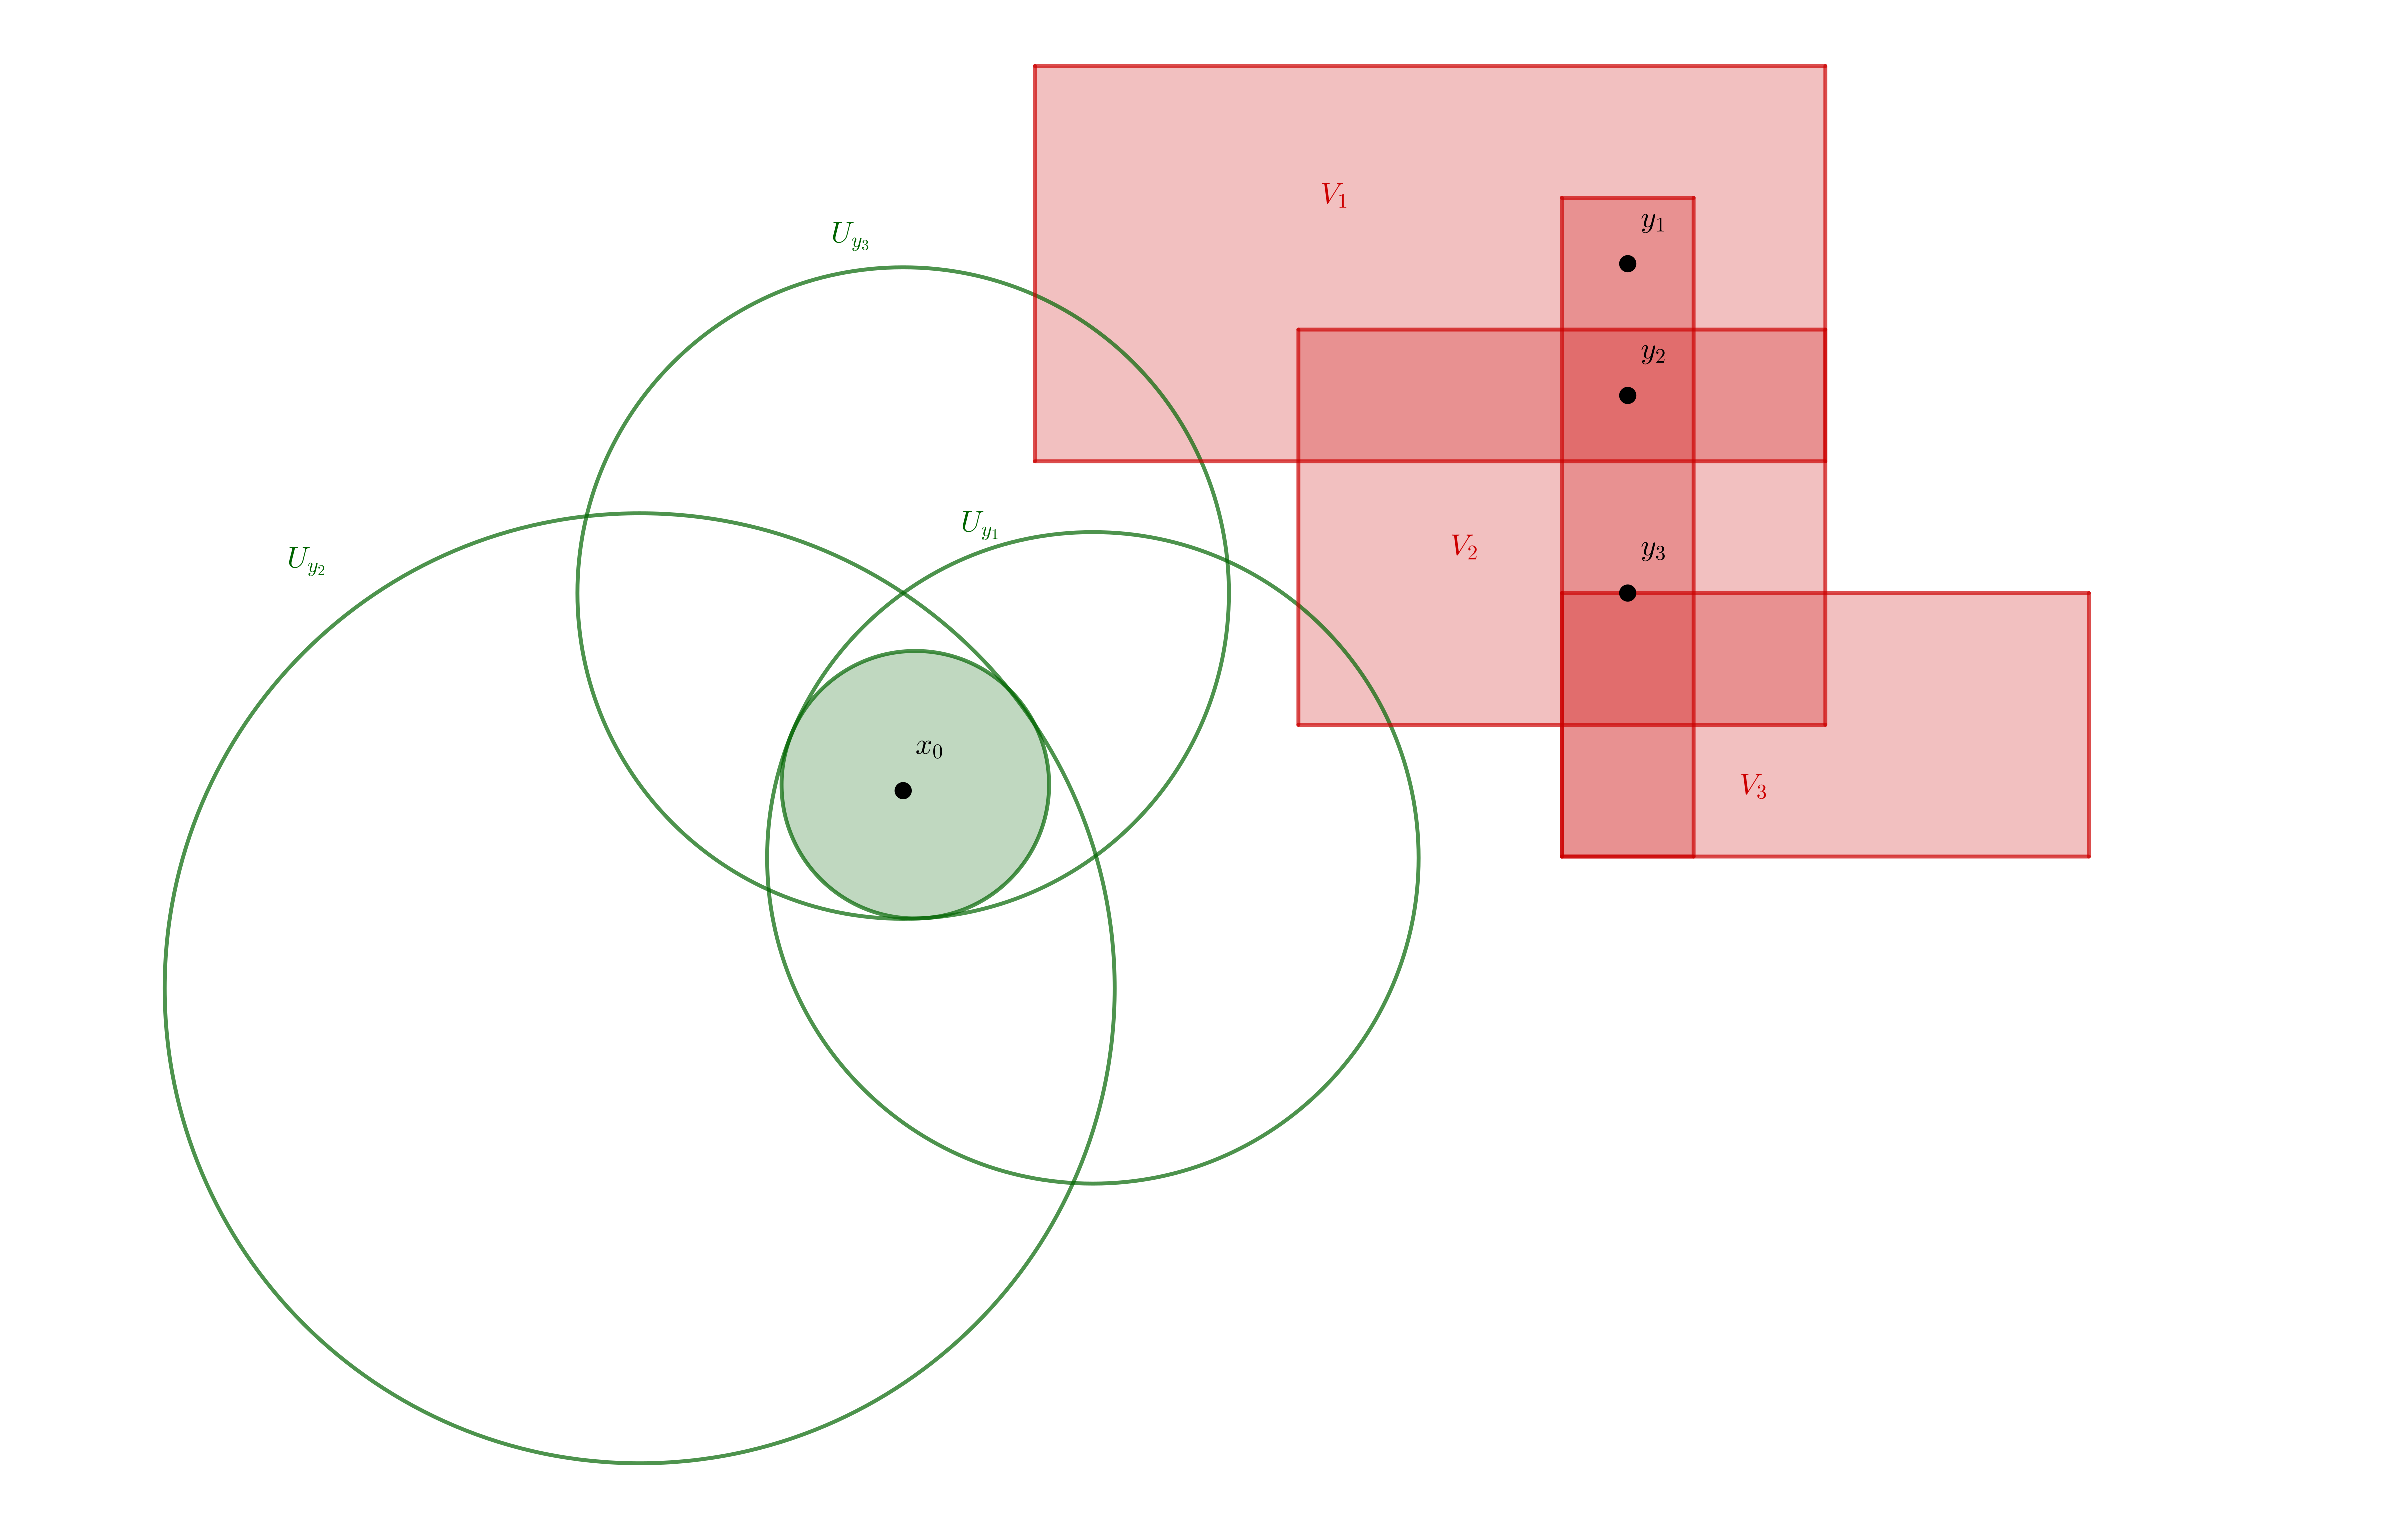
\includegraphics[scale=0.2]{Figures/Chapter3/compactHausdorff1.eps}
    \caption{}
    \label{fig_3.1}
\end{figure}

\begin{corollary}
    If $Y$ is a compact subspace of a Hausdorff space $X$, and  $ x_0 \in \com{X}{Y}$, then there
    exists opensets $U$ and  $V$ in  $X$ with  $ x_0 \in U$ and $Y \subseteq V$, respectively.
\end{corollary}

%----------------------------------------------------------------------------------------
%	SECTION 1.1
%----------------------------------------------------------------------------------------

\section{Modules.}
\label{section1}



\end{document}
